% Technical report: hardware-aware multi-objective compression, objectives {loss, decode latency, memory}.
% Build from this folder:  latexmk -pdf main.tex
%                     or:  pdflatex main && bibtex main && pdflatex main && pdflatex main
\documentclass[11pt]{article}
\usepackage[margin=1in]{geometry}
\usepackage[T1]{fontenc}
\usepackage{lmodern}
\usepackage{amsmath,amssymb}
\usepackage{booktabs}
\usepackage{array}
\usepackage{microtype}
\usepackage{graphicx}
\usepackage{subcaption}
\usepackage{xcolor}
\usepackage{tikz}
\usetikzlibrary{arrows.meta,positioning}
\usepackage{enumitem}
\usepackage[numbers,sort&compress]{natbib}
\usepackage[hidelinks]{hyperref}

\newcommand{\dloss}{\Delta\mathcal{L}}
\newcolumntype{P}[1]{>{\raggedright\arraybackslash}p{#1}}
% pipeline figure: one color per stage (the blue, aqua and orange of the plots)
\definecolor{cprep}{HTML}{7A8699}
\definecolor{csearch}{HTML}{2A78D6}
\definecolor{ceval}{HTML}{1BAF7A}
\definecolor{cfinal}{HTML}{EB6834}
\newcommand{\us}{\,$\mu$s}
\setlist{itemsep=2pt, topsep=4pt}

\title{Hardware-Aware Multi-Objective Compression of Language Models:\\
Minimizing Loss, Decode Latency and Memory Together}
\author{Rasa Khosrowshahli}
\date{October 2026}

\begin{document}
\maketitle

\begin{abstract}
Our earlier evolutionary compression search traded the loss of a language model against a storage
size computed from idealized encodings, and it evaluated accuracy on a fake-quantized model whose
weights are written back as dense bf16 tensors. Neither quantity changes how fast the model runs: a
fake-quantized matrix takes exactly as long to multiply as the original, and unstructured sparsity at
the levels the search produces is slower than dense on a GPU. This report describes a redesigned,
hardware-aware search in which every candidate is a model the target GPU can execute faster. The
decision variables are the weight format (bf16, or int4 with groups of 32, 64 or 128 weights) of each
matrix role in each depth band, the format of the output head, the fraction of MLP neurons kept per
band, and the number of attention and MLP sublayers removed. Parameters that change accuracy but not
cost, such as the clipping range of each int4 group, are solved per group instead of being searched.
The latency objective is the GPU time of one decode step, predicted from a table of kernel times
measured on the target GPU; the memory objective is the deployed footprint of weights, scales and KV
cache. On Qwen2.5-0.5B-Instruct and an NVIDIA RTX 3060, the latency model predicts the profiled kernel
time of the deployed models within $\pm1.1\%$, and the simulated loss matches the loss with the real
int4 kernel within 0.0024 nats. Uniform int4 halves the decode time ($6.78\rightarrow3.4$--$3.6$\,ms)
at a loss increase of 0.08--0.18 nats; further speed comes only from structural pruning, at a much
larger loss. A two-objective search with objectives \{loss, latency\} (memory as a constraint) and a
three-objective search with objectives \{loss, latency, memory\} and the same budget produce nearly the
same front (three-objective
hypervolume 0.3655 vs 0.3646), because latency and memory are almost collinear on this model; the
two-objective search converged faster in every objective space.
\end{abstract}

\tableofcontents

% =====================================================================================================
\section{Introduction}

Post-training compression of language models is usually judged by the size of the compressed weights
and by perplexity. What a deployment pays for, however, is the time to generate each token and the GPU
memory the model occupies. Both fall only when the model is stored and executed in formats for which
fast kernels exist, so a compression search that targets them has to know which formats the target GPU
can execute and how fast.

Our previous search applied uniform binning quantization (UBQ),
optionally followed by entropy-constrained merging of the levels (UBQ-ECSQ), with four or five genes
shared by every matrix of the model: the number of grid levels $k$, a clipping factor $c$, a pruning
interval $[\alpha,\beta]$ in units of the row's standard deviation, and the merge ratio $\rho$. Its
second objective was the encoded size of the weights in the smallest of several storage formats
(dense codes, a bitmap of non-zeros, CSR, or entropy-coded codes). Section~\ref{sec:motivation}
shows with measurements why this formulation cannot trade accuracy for speed: the compressed weights
are evaluated as dense bf16 tensors, which run at the original speed; the storage formats have no fast
decoding kernels; and unstructured pruning at the sparsity the search produces is slower than a dense
matrix product.

This report describes a hardware-aware redesign built on four principles:
\begin{enumerate}
  \item \textbf{Every candidate is executable.} The search space contains only formats with a kernel on
        the target GPU (a ``kernel menu''); every configuration can be built and timed.
  \item \textbf{Genes are the choices that change cost.} Parameters that change only accuracy at a fixed
        cost, such as the clipping range of a quantization group, have a single best value per layer and
        are solved deterministically inside the evaluation.
  \item \textbf{Latency comes from a measured table, not from a stopwatch in the loop.} Kernel times
        are measured once per GPU and summed per configuration, which makes the objective deterministic
        and cheap.
  \item \textbf{Decisions are per layer group,} since layers differ both in sensitivity and in how much
        time their matrices take.
\end{enumerate}

\noindent The contributions are:
\begin{itemize}
  \item a decision space of 23 integer genes for Qwen2.5-0.5B (24 for nanochat d34) mixing int4
        quantization, MLP width pruning and sublayer removal, with per-group clipping solved by an inner
        solver (Sections~\ref{sec:formulation} and~\ref{sec:operators});
  \item an additive decode-latency model built from CUDA-graph kernel timings and profiler-calibrated
        overheads, validated against the deployed models within $\pm1.1\%$, and a memory model of the
        deployed footprint (Section~\ref{sec:cost});
  \item an NSGA-II search with two variants, objectives \{loss, latency\} under a memory constraint and
        objectives \{loss, latency, memory\} (Section~\ref{sec:search});
  \item a study on Qwen2.5-0.5B-Instruct on an RTX 3060 comparing the two variants by hypervolume
        (Section~\ref{sec:experiments}).
\end{itemize}

% =====================================================================================================
\section{Motivation: what the GPU can accelerate}
\label{sec:motivation}

All measurements in this report were made on an NVIDIA GeForce RTX 3060 8\,GB (Ampere, compute
capability 8.6, 28 SMs, 1.5\,MB L2 cache, 128-bit GDDR6 at 15\,Gb/s, i.e.\ 240\,GB/s), with PyTorch
2.13 and CUDA 12.6 on Windows 11, using only kernels that ship with PyTorch (no Triton, torchao, vLLM or
FLUTE).

\paragraph{Fake quantization does not change latency.}
The search wrote the dequantized weights back into the dense bf16 matrices, and the forward pass
multiplies them with a dense cuBLAS kernel, which reads every 16-bit weight whatever its value.
Table~\ref{tab:fakequant} confirms that a matrix with 3 distinct values and 93\% zeros is multiplied
exactly as fast as the original.

\begin{table}[htbp]
\centering
\small
\begin{tabular}{lrrr}
\toprule
Weights of an $8704\times2176$ matrix (d34 MLP) & Zeros & Batch 1 (\us) & Batch 2048 (\us) \\
\midrule
Original bf16                              & 0\%  & 175.6   & 3092 \\
UBQ, $k=256$                               & 1\%  & 171.3   & 3053 \\
UBQ, $k=16$                                & 21\% & 175.9   & 3055 \\
UBQ, $k=3$ with interval pruning           & 93\% & 176--181 & 3059--3140 \\
\bottomrule
\end{tabular}
\caption{Time of one bf16 matrix product with fake-quantized weights (mean over 500 calls). The values
of the weights do not affect a dense kernel.}
\label{tab:fakequant}
\end{table}

\paragraph{The kernel menu.}
Table~\ref{tab:menu} times the formats that could reduce latency on the four matrix shapes of nanochat
d34 (attention $2176\times2176$, MLP $8704\times2176$ and $2176\times8704$, output head
$65536\times2176$) at a decode batch of 1 and 16 tokens and at a 2048-token prompt.
\begin{table}[htbp]
\centering
\footnotesize
\begin{tabular}{P{4.3cm}cccP{2.6cm}}
\toprule
Format & Batch 1 & Batch 16 & 2048 tokens & On this machine \\
\midrule
bf16 with 25\% of the rows removed (structured) & 1.24--1.35$\times$ & 1.29--1.78$\times$ & 1.28--1.64$\times$ & yes, dense kernel \\
int4 weight-only, group 128 (tinygemm)          & 2.91--3.76$\times$ & 1.51--1.83$\times$ & 0.19--0.32$\times$ & yes, built into PyTorch \\
int8 weights and activations (eager)            & 0.20--1.60$\times$ & 0.27--1.48$\times$ & 0.50--0.77$\times$ & matmul only \\
int8 matrix product alone                       & --                 & --                 & 1.78--2.86$\times$ & needs a fused kernel \\
bf16 2:4 semi-structured sparsity               & --                 & --                 & --                 & no \\
CSR, 50\% unstructured zeros                    & 0.22--0.42$\times$ & $\le$0.02$\times$  & --                 & yes \\
CSR, 90\% unstructured zeros                    & 0.59--2.01$\times$ & 0.09--0.27$\times$ & --                 & yes \\
\bottomrule
\end{tabular}
\caption{Speedup over a bf16 matrix product, as the range over the four d34 matrix shapes. Values below
1 are slowdowns. The int8 row with activations quantizes them in eager PyTorch, outside the kernel; the
row below it times the int8 tensor-core product alone. 2:4 sparsity needs CUTLASS sparse kernels or
cuSPARSELt, which the Windows build of PyTorch does not include.}
\label{tab:menu}
\end{table}

\noindent Summed over d34's 34 blocks and output head, the matrix products of one decode step take
20.1\,ms in bf16 (the dense kernels reach about 220\,GB/s, 92\% of the peak bandwidth), 7.1\,ms with
int4 blocks and a bf16 head, and 6.1\,ms with int4 everywhere ($3.3\times$). Four consequences shape the
design:
\begin{itemize}
  \item \textbf{Speedup depends on the workload.} Weight-only int4 is a large win when decoding one
        token at a time, which is limited by the bytes read from memory, and a 3--5$\times$ loss on long
        prompts, which are limited by compute. A latency objective is therefore defined for a workload.
  \item \textbf{Unstructured pruning does not buy speed} at the sparsity the earlier search reached;
        only structured pruning (rows, neurons, whole sublayers) or 2:4 patterns do.
  \item \textbf{Kernels execute fixed code widths.} A grid of $k=37$ levels needs 6-bit codes and uses
        37 of their 64 values; deployable formats use all $2^b$ levels of a supported width $b$.
  \item \textbf{Latency and memory are correlated when decoding,} because time is roughly the bytes
        read divided by the bandwidth. They diverge for memory that is not read per token (an embedding
        table, of which a lookup reads one row) and for the KV cache.
\end{itemize}

% =====================================================================================================
\section{Problem formulation}
\label{sec:formulation}

\subsection{Model structure}
The search applies to HuggingFace Llama/Qwen2-style models and to nanochat GPT models
\cite{karpathy2025nanochat}. A model has $L$ blocks, each with an attention sublayer (projections $q$,
$k$, $v$ and the output projection $o$) and an MLP sublayer (an up projection, which is the pair gate and
up in a SwiGLU MLP, and a down projection), followed by an output head. Matrices are grouped by
\emph{role} $r\in\{\text{qkv},\text{o},\text{up},\text{down}\}$ and \emph{depth band}
$b\in\{1,\dots,B\}$, the layers split into $B$ equal runs. The $q$, $k$ and $v$ projections share a
format because deployments fuse them into one product, and so do gate and up.

Qwen2.5-0.5B-Instruct \cite{qwen2025qwen25} has $L=24$ blocks of width $d=896$, 14 query heads and 2
key-value heads of dimension 64 (grouped-query attention), a SwiGLU MLP of width $I=4864$, and a
vocabulary of 151{,}936 tokens whose embedding is tied to the output head (136\,M of its 494\,M
parameters). All 493{,}961{,}216 matrix weights are compressible; the remaining 43{,}904 parameters are
normalization weights.

\subsection{Decision variables}
Table~\ref{tab:genes} lists the genes. All are integers that index an ordered list of options, so that a
step of one changes the option to its neighbor.

\begin{table}[htbp]
\centering
\small
\begin{tabular}{P{1.6cm}P{3.6cm}P{3.6cm}cP{3.6cm}}
\toprule
Gene & Granularity & Options & Count & What it changes \\
\midrule
$f_{r,b}$ & role $\times$ band ($4\times4$) & bf16, int4 group 32, 64, 128 & 16 & bytes read per token, memory \\
$f_{\text{head}}$ & output head (with a tied embedding) & as above & 1 & the largest single product \\
$f_{\text{emb}}$ & untied embeddings (d34 only) & as above & 0 (1) & memory only \\
$\kappa_b$ & MLP width per band & $1, \tfrac78, \tfrac34, \tfrac58, \tfrac12$ & 4 & every regime \\
$s_{\text{attn}}$ & attention sublayers removed & $0,\dots,L/4$ & 1 & products, attention, KV cache \\
$s_{\text{mlp}}$ & MLP sublayers removed & $0,\dots,L/4$ & 1 & products \\
\bottomrule
\end{tabular}
\caption{Genes of the hardware-aware search: 23 for Qwen2.5-0.5B, 24 for nanochat d34.}
\label{tab:genes}
\end{table}

\noindent The kept MLP width of a band is $n_b=128\cdot\operatorname{round}(\kappa_b I/128)$ neurons, a
multiple of 128 so that the pruned matrices keep tensor-core-friendly shapes and whole int4 groups. With
$B=4$ bands and at most $L/4=6$ removals, the Qwen search space has
$4^{17}\cdot5^{4}\cdot7^{2}\approx5.3\times10^{14}$ configurations; for d34 ($L=34$, an untied
embedding) it has $4^{18}\cdot5^{4}\cdot9^{2}\approx3.5\times10^{15}$.

\subsection{What is solved instead of searched}
Three choices change accuracy but not cost, so they are made by deterministic procedures computed once
or cached per matrix (Section~\ref{sec:operators}):
\begin{itemize}
  \item the clipping range of each int4 group, chosen from six ratios by an activation-weighted error;
  \item which MLP neurons are kept, ranked by a Wanda-style importance score \cite{sun2024wanda};
  \item which sublayers are removed first, ranked once by the loss increase of removing each alone.
\end{itemize}

\subsection{Objectives and constraints}
Let $x$ be a gene vector and $\theta_x$ the model it describes. The accuracy objective is the increase
of the mean next-token cross-entropy on a fixed calibration batch $D$,
\begin{equation}
  \dloss(x) = \mathcal{L}_D(\theta_x) - \mathcal{L}_D(\theta_0),\qquad
  \mathcal{L}_D(\theta) = -\frac{1}{|D|}\sum_{t\in D}\log p_\theta(x_{t+1}\mid x_{\le t}),
\end{equation}
measured in nats per token; a difference of $\dloss$ nats is a perplexity ratio of $e^{\dloss}$. With
the decode latency $T(x)$ and the deployed memory $M(x)$ of Section~\ref{sec:cost}, the two scenarios are
\begin{align}
  \text{2 objectives:}\quad & \min_x\ \big(\dloss(x),\,T(x)\big)
     && \text{s.t. } \dloss(x)\le1,\ M(x)\le M_{\max}, \\
  \text{3 objectives:}\quad & \min_x\ \big(\dloss(x),\,T(x),\,M(x)\big)
     && \text{s.t. } \dloss(x)\le1,\ M(x)\le M_{\max}.
\end{align}
With a single target GPU, memory matters first as a constraint: a model that fits gets no faster by
shrinking further. As an objective it adds the trade-off between memory and latency where the two
diverge. Both scenarios log $M(x)$ for every solution, so their fronts can be compared in all three
objectives.

% =====================================================================================================
\section{Compression operators}
\label{sec:operators}

\subsection{int4 group quantization}
The int4 format is the one consumed by PyTorch's built-in tinygemm kernel (compute capability 8.0 and
above; also used by torchao \cite{torchao2024}). A matrix $W\in\mathbb{R}^{N\times K}$ is split into groups of $g$ consecutive
weights of a row. For a group $G$ with range $[w_{\min},w_{\max}]$ and a clipping ratio $\gamma$,
\begin{align}
  s_\gamma &= \operatorname{bf16}\!\Big(\frac{\gamma\,(w_{\max}-w_{\min})}{15}\Big), \qquad
  z_\gamma = \operatorname{bf16}\big(\gamma\,w_{\min} + 8\,s_\gamma\big), \\
  q_j &= \operatorname{clip}\!\Big(\operatorname{round}\Big(\frac{w_j - z_\gamma}{s_\gamma}\Big)+8,\ 0,\ 15\Big),
  \qquad \hat w_j = (q_j-8)\,s_\gamma + z_\gamma ,
\end{align}
so that $q=0$ and $q=15$ reconstruct $\gamma w_{\min}$ and $\gamma w_{\max}$. The ratio of each group is
\begin{equation}
  \gamma^\star = \arg\min_{\gamma\in\{1,0.95,0.9,0.85,0.8,0.75\}}\ \sum_{j\in G}\mathbb{E}\big[x_j^2\big]\,\big(w_j-\hat w_j(\gamma)\big)^2 ,
\end{equation}
where $\mathbb{E}[x_j^2]$ is the second moment of input channel $j$ on the calibration batch. This is the
output error $\mathbb{E}\lVert(W-\hat W)x\rVert^2$ under a diagonal approximation of $\mathbb{E}[xx^\top]$,
in the spirit of the clipping search of AWQ \cite{lin2024awq}. Error-compensating quantizers such as GPTQ
\cite{frantar2023gptq} fit the same slot and are left for later. A group of $g$ weights costs
$g/2$ bytes of codes plus 4 bytes of scale and zero, i.e.\ $4+32/g$ bits per weight.

\subsection{MLP width pruning}
Neuron $j$ of block $\ell$ is scored by $\lVert W^{\text{down}}_{\ell,:,j}\rVert_2\sqrt{\mathbb{E}[h_{\ell,j}^2]}$,
the norm of its output weights times the root mean square of its activation $h$ (the input of the down
projection), as in Wanda \cite{sun2024wanda} aggregated per neuron (see also LLM-Pruner
\cite{ma2023llmpruner}). The $n_b$ highest-scoring neurons are kept: the deployed model slices the rows
of gate and up and the columns of down. In the search, the removed rows and columns are set to zero
instead. For the down projection, the int4 groups are formed over the kept columns only, exactly as in
the sliced matrix.

\subsection{Sublayer removal}
Removing a sublayer means that it adds nothing to the residual stream; in the search this is done by
zeroing its output projection ($o$ or down), which none of the supported models follows with a bias. The
order of removal is fixed once: each of the $2L$ sublayers is removed alone and the loss increase is
measured on 4 calibration windows, then $s_{\text{attn}}$ removes the first $s_{\text{attn}}$ attention
sublayers of this ranking and $s_{\text{mlp}}$ the first MLP sublayers, as in ShortGPT
\cite{men2024shortgpt} with a direct loss criterion. Appendix~\ref{app:removal} lists the ranking for
Qwen2.5-0.5B. Reducing $L$ binary genes to one integer per kind keeps the genome small.

\subsection{The simulated model is the deployed model}
The search evaluates the loss with the deployed weights written into the model: dequantized int4 values,
zeroed neurons and zeroed output projections. The deployed model is built separately: int4 matrices on
the tinygemm kernel, MLPs sliced to the kept neurons and removed sublayers replaced by a module that
returns zeros. On small random Qwen2 and nanochat models the two agree exactly for pruning and removal
in bf16, and to bf16 rounding (relative error below $3\times10^{-2}$ on the logits) with the int4 kernel. On the real model the calibration loss of the
simulated and deployed models differ by at most 0.0024 nats on all validated points
(Table~\ref{tab:validation}).

% =====================================================================================================
\section{Cost models}
\label{sec:cost}

\subsection{Memory}
A matrix of $N\times K$ weights takes $B(N,K,\text{bf16})=2NK$ bytes, or
$B(N,K,\text{int4}_g)=NK/2+4N\,K/g$ bytes. The deployed memory of configuration $x$ for $\beta$ sequences
of $C$ tokens of context is
\begin{equation}
  M(x) = 2P_{\text{rest}} + \sum_{m\in\mathcal{M}(x)}\Big(B(N_m,K_m,f_m)+2N_m\,\mathbb{1}[\text{bias}_m]\Big)
       + \beta\, C\,\big(L-|A(x)|\big)\cdot 2H_{kv}d_h\cdot 2 ,
\end{equation}
where $\mathcal{M}(x)$ are the matrices that remain (pruned to their kept shape), $P_{\text{rest}}$ the
remaining parameters in bf16, $A(x)$ the removed attention sublayers, and the last term the bf16 keys and
values of the attention sublayers that remain. A tied embedding is counted once with the output head.
For the uncompressed Qwen model at $\beta=1$, $C=1024$ this gives 988.1\,MB of weights and 12.6\,MB of
KV cache.

\subsection{Decode latency}
The latency objective is the GPU time of one decode step for $\beta$ sequences at $C$ tokens of
context, as a runtime without launch overhead (CUDA graphs) would see it:
\begin{equation}
\begin{aligned}
  T(x) = T_{\text{fixed}}
   &+ \sum_{\ell\notin A(x)}\Big(T^{\text{attn}}_{\text{misc}} + T_{\text{attn}}(\beta,C)
        + \sum_{m\in\{q,k,v,o\}} t\big(N_m,K_m,f_m\big)\Big) \\
   &+ \sum_{\ell\notin U(x)}\Big(T^{\text{mlp}}_{\text{misc}}
        + \sum_{m\in\text{up}_\ell} t\big(n_{b(\ell)},d,f_m\big) + t\big(d,n_{b(\ell)},f_{\text{down}}\big)\Big)
   + t\big(V,d,f_{\text{head}}\big),
\end{aligned}
\label{eq:latency}
\end{equation}
where $U(x)$ are the removed MLP sublayers and $t(N,K,f)$ the measured time of a product of $\beta$ tokens
with an $N\times K$ matrix in format $f$.

\paragraph{Matrix products.}
$t$ is measured once for every shape the deployed model can contain (all kept MLP widths included) and
every format. Each measurement captures $n$ calls in a CUDA graph, cycling through $c$ copies of the
weight with $c=\min(16,\lceil4\,\text{L2}/\text{bytes}\rceil)$ so that the copies do not fit in the L2
cache together, as in the model, where every layer reads its own weights from memory. $n$ is chosen so
that one replay takes about 2\,ms, which keeps the GPU at full clocks; the time is the minimum over 15
replays, since other work on the GPU can only slow a replay down. The GPU is warmed up for one second
before the table is measured. A format whose kernel cannot run a shape falls back to bf16 for that shape.

\paragraph{Attention.}
$T_{\text{attn}}$ is the faster of PyTorch's scaled-dot-product attention and a plain grouped-query
implementation (two batched matrix products in which each query head reads its key-value head in place).
Builds without FlashAttention \cite{dao2024flashattention2}, such as this Windows build, run SDPA's math
path for grouped-query attention, which expands the cache: at 1024 tokens of context for Qwen it takes
130.6\us{} per layer against 19.9\us{} for the grouped implementation.

\paragraph{Everything else.}
Norms, rotary embeddings, activations, residual additions, the embedding lookup and the logits are
calibrated on the real model. The profiler's summed kernel durations of one forward pass of $\beta$
tokens without a cache (the fastest of three, after a warm-up) are measured for the full model
($T_{\text{full}}$), with every attention sublayer removed ($T_{\text{no-attn}}$) and with every MLP
sublayer removed ($T_{\text{no-mlp}}$). Then
\begin{align}
  T^{\text{attn}}_{\text{misc}} &= \frac{T_{\text{full}}-T_{\text{no-attn}}-\sum_{\text{attn}}t^{\text{bf16}}}{L} - T^{\text{own}}_{\text{attn}}(\beta,1), \\
  T^{\text{mlp}}_{\text{misc}}  &= \frac{T_{\text{full}}-T_{\text{no-mlp}}-\sum_{\text{mlp}}t^{\text{bf16}}}{L}, \qquad
  T_{\text{fixed}} = T_{\text{no-attn}}+T_{\text{no-mlp}}-T_{\text{full}}-t^{\text{bf16}}_{\text{head}},
\end{align}
each clamped at zero, where $T^{\text{own}}_{\text{attn}}(\beta,1)$ is the model's own attention over one
token. By construction, Eq.~\eqref{eq:latency} then reproduces the profiled time of the uncompressed
model. For Qwen: $T_{\text{full}}=6772.6$\us, $T_{\text{no-attn}}=5070.0$\us, $T_{\text{no-mlp}}=3570.2$\us,
hence $T^{\text{attn}}_{\text{misc}}=23.8$\us, $T^{\text{mlp}}_{\text{misc}}=6.0$\us{} and
$T_{\text{fixed}}=666.0$\us. Appendix~\ref{app:table} lists the measured product times. The
approach is that of latency lookup tables in hardware-aware architecture search
\cite{cai2019proxylessnas,wu2019fbnet} and mixed-precision quantization \cite{wang2019haq,yao2021hawqv3}.

\subsection{Anatomy of a decode step}
Table~\ref{tab:anatomy} decomposes the predicted decode step of Qwen2.5-0.5B. In bf16 the MLP products
take 45\% of the time and the output head 18\%. With int4 everywhere the products shrink by
3--4$\times$, and attention, the per-sublayer operations and the fixed part become 55\% of the step. They
bound what weight compression alone can achieve: $6783/1859\approx3.6\times$.

\begin{table}[htbp]
\centering
\small
\begin{tabular}{lrrrr}
\toprule
& \multicolumn{2}{c}{bf16} & \multicolumn{2}{c}{int4, group 128} \\
\cmidrule(lr){2-3}\cmidrule(lr){4-5}
Part of the step & \us & share & \us & share \\
\midrule
MLP products (gate, up, down) $\times24$          & 3060 & 45\% & 859  & 26\% \\
Attention products ($q,k,v,o$) $\times24$          & 662  & 10\% & 314  & 9\% \\
Attention over 1024 cached tokens $\times24$       & 478  & 7\%  & 478  & 14\% \\
Output head ($151936\times896$)                    & 1202 & 18\% & 321  & 10\% \\
Norms, rotary, activations, residuals $\times24$   & 715  & 11\% & 715  & 21\% \\
Fixed (embedding, final norm, logits)              & 666  & 10\% & 666  & 20\% \\
\midrule
Total                                              & 6783 &      & 3353 &      \\
\bottomrule
\end{tabular}
\caption{Predicted GPU time of one decode step of Qwen2.5-0.5B-Instruct (batch 1, 1024 tokens of
context) on the RTX 3060.}
\label{tab:anatomy}
\end{table}

\subsection{Validation against the deployed models}
After each search, six points of the final front and the uncompressed model are built as deployed
models. One forward pass of a single token (the shape the overheads were calibrated on) is profiled
and compared with Eq.~\eqref{eq:latency} evaluated for that shape.
Table~\ref{tab:validation} shows the results for both searches of Section~\ref{sec:experiments}. The
prediction is within $-0.7\%$ to $+1.1\%$ of the measured GPU time, including configurations with
pruned MLPs and up to 10 removed sublayers. The last two columns compare the calibration loss (on two
windows) of the simulated and the deployed model.

The same table shows the wall-clock time of the forward pass in eager PyTorch: 23--35\,ms whatever the
configuration, because a HuggingFace forward of a 0.5\,B model at batch 1 is limited by Python and
kernel-launch overhead, not by the GPU. The speedups predicted here are realized by runtimes without
that overhead (CUDA graphs, compiled execution, or a serving engine).

\begin{table}[htbp]
\centering
\footnotesize
\setlength{\tabcolsep}{4pt}
\begin{tabular}{lP{5.0cm}rrrrrr}
\toprule
& & \multicolumn{2}{c}{GPU time (ms)} & & Eager & \multicolumn{2}{c}{Loss (nats)} \\
\cmidrule(lr){3-4}\cmidrule(lr){7-8}
Search & Configuration & predicted & measured & error & (ms) & simulated & deployed \\
\midrule
2 obj. & uncompressed                                         & 6.77 & 6.79 & $-0.2\%$ & 28.0 & 2.8926 & 2.8926 \\
       & mixed int4, MLP $\tfrac78$ in 2 bands, $-6$ attn, $-4$ MLP & 2.85 & 2.82 & $+1.0\%$ & 23.1 & 3.7105 & 3.7110 \\
       & mixed bf16/int4, MLP $\tfrac78$ in 1 band, $-6$ attn  & 3.15 & 3.13 & $+0.6\%$ & 23.2 & 3.3420 & 3.3428 \\
       & int4 group 32 everywhere                              & 3.56 & 3.52 & $+1.1\%$ & 29.7 & 2.9784 & 2.9781 \\
       & mixed bf16/int4 (8.3 bits per weight)                 & 4.60 & 4.60 & $0.0\%$  & 28.2 & 2.9467 & 2.9456 \\
       & mostly bf16 (12.3 bits per weight)                    & 5.72 & 5.72 & $-0.1\%$ & 26.7 & 2.9147 & 2.9137 \\
\midrule
3 obj. & uncompressed                                         & 6.77 & 6.80 & $-0.4\%$ & 34.6 & 2.8926 & 2.8926 \\
       & int4 group 128, MLP $\tfrac12$ in 1 band, $-5$ attn   & 2.97 & 2.96 & $+0.3\%$ & 27.2 & 3.4952 & 3.4958 \\
       & mixed int4, MLP $\tfrac12$ in 2 bands, $-3$ MLP       & 3.14 & 3.10 & $+1.1\%$ & 31.7 & 3.6098 & 3.6122 \\
       & int4, mostly group 128                               & 3.39 & 3.36 & $+0.9\%$ & 33.2 & 3.0372 & 3.0386 \\
       & mixed bf16/int4 (8.3 bits per weight)                 & 4.52 & 4.51 & $+0.1\%$ & 31.6 & 2.9489 & 2.9494 \\
       & mostly bf16 (12.8 bits per weight)                    & 5.84 & 5.86 & $-0.4\%$ & 32.9 & 2.9091 & 2.9095 \\
\bottomrule
\end{tabular}
\caption{Predicted against measured GPU time of the deployed models (one token, batch 1), eager
wall-clock time, and calibration loss of the simulated against the deployed model.}
\label{tab:validation}
\end{table}

\subsection{Measurement pitfalls}
Four effects can make such a table wrong by up to $2\times$; the measurement handles each of them.
\begin{itemize}
  \item \textbf{Attention fallback.} Without FlashAttention, SDPA's math path made Qwen's attention
        $6.6\times$ slower than necessary and would have made removing attention look far more valuable
        than on a reasonable runtime. The table takes the fastest available implementation.
  \item \textbf{Clock drift and contention.} An idle GPU runs its memory clock far below the maximum,
        and kernels of a few microseconds timed in short bursts varied by 20--40\%; another process on
        the GPU slowed some measurements and not others. Warm-up, replays of about 2\,ms and the minimum
        over replays brought run-to-run differences below 1\%. The table must be measured on an
        otherwise idle GPU: the overhead terms are differences of profiles, and contention distorts them.
  \item \textbf{L2 reuse.} Timing one small matrix repeatedly measures the L2 cache, not memory;
        cycling through copies larger than the cache removes this.
  \item \textbf{Eager overhead.} Wall-clock timing of eager forwards measures the CPU, not the GPU
        (Table~\ref{tab:validation}); the profiler's kernel durations measure the GPU.
\end{itemize}

% =====================================================================================================
\section{Search algorithm}
\label{sec:search}

The search is NSGA-II \cite{deb2002nsga2}, implemented with pymoo \cite{blank2020pymoo}
(Figure~\ref{fig:pipeline}).
\begin{itemize}
  \item \textbf{Encoding and operators.} Genes are integers in $[0,n_i-1]$. Simulated binary crossover
        (probability 0.9, $\eta=3$) and polynomial mutation ($\eta=3$, per-variable probability
        $1/23$) act on real values that are rounded back to integers; the small distribution index gives
        steps of more than one option.
  \item \textbf{Initial population.} The first four individuals use one format everywhere (bf16, which
        is the original model, and int4 with groups of 32, 64 and 128) with nothing pruned. The others
        are random, except that each structural gene ($\kappa_b$, $s_{\text{attn}}$, $s_{\text{mlp}}$)
        is zero with probability $1/2$, since random pruning mostly breaks the model.
  \item \textbf{Duplicates and constraints.} Offspring that decode to an existing configuration are
        regenerated. Constraints use NSGA-II's constrained dominance: feasible solutions first,
        infeasible ones by their violation.
  \item \textbf{Evaluation.} An evaluation writes the configuration into the model, measures the
        calibration loss, restores the original weights and evaluates $T(x)$ and $M(x)$ analytically.
  \item \textbf{Hypervolume.} The hypervolume \cite{zitzler1999hypervolume} of each generation's front
        is normalized by the nadir of the first feasible front, with reference point $(1,\dots,1)$.
\end{itemize}

\begin{figure}[htbp]
\centering
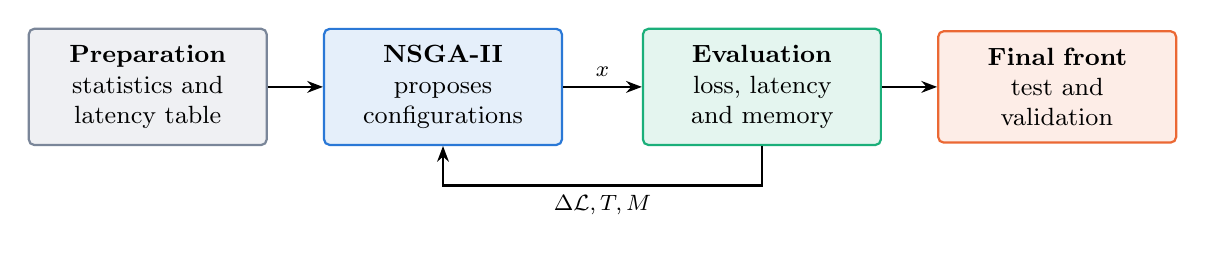
\begin{tikzpicture}[
  box/.style={draw, line width=0.8pt, rounded corners=2pt, align=center, font=\small, text width=2.6cm,
              inner sep=6pt, minimum height=1.4cm},
  arr/.style={-{Stealth[length=2mm]}, thick},
  lab/.style={font=\footnotesize},
  node distance=7mm]
\node[box, draw=cprep, fill=cprep!12] (prep) {\textbf{Preparation}\\statistics and\\latency table};
\node[box, draw=csearch, fill=csearch!12, right=of prep] (nsga) {\textbf{NSGA-II}\\proposes\\configurations};
\node[box, draw=ceval, fill=ceval!12, right=10mm of nsga] (eval) {\textbf{Evaluation}\\loss, latency\\and memory};
\node[box, draw=cfinal, fill=cfinal!12, right=of eval] (final) {\textbf{Final front}\\test and\\validation};
\draw[arr] (prep) -- (nsga);
\draw[arr] (nsga) -- node[lab, above] {$x$} (eval);
\draw[arr] (eval.south) -- ++(0,-0.5) -| node[lab, pos=0.25, below] {$\dloss, T, M$} (nsga.south);
\draw[arr] (eval) -- (final);
\end{tikzpicture}
\caption{Pipeline of the hardware-aware search. Before the search, the activation statistics, the
sublayer removal ranking and the latency table of the GPU are computed once. NSGA-II proposes
configurations $x$; each is evaluated by its calibration loss $\dloss$ and its predicted latency $T$ and
memory $M$. The final front is scored on test sets and validated with deployed models.}
\label{fig:pipeline}
\end{figure}

% =====================================================================================================
\section{Experiments on Qwen2.5-0.5B-Instruct}
\label{sec:experiments}

\subsection{Setup}
\begin{itemize}
  \item \textbf{Calibration.} One fixed batch of 8 windows of 2048 tokens of C4 train \cite{raffel2020c4};
        the uncompressed model's loss on it is 2.8854 nats.
  \item \textbf{Workload.} Decoding one sequence at 1024 tokens of context; the uncompressed model's
        predicted step takes 6.78\,ms and needs 1000.6\,MB.
  \item \textbf{Constraints.} $\dloss\le1$ nat and $M\le7000$\,MB. The memory constraint never binds:
        the uncompressed model needs 1001\,MB.
  \item \textbf{Budget.} A population of 40 for 12 generations (480 evaluations) and seed 42 for both
        scenarios, which therefore start from the same initial population. An evaluation takes about
        4.4\,s, a generation about 175\,s, a search about 36 minutes.
  \item \textbf{Preparation.} Activation statistics (4\,s), the removal ranking (96 evaluations on 4
        windows, 99\,s) and the latency table (7\,s) are computed once per run.
  \item \textbf{Test.} Six points of each final front, spread evenly by latency, are scored on 32
        windows of 2048 tokens of WikiText-2 test \cite{merity2017wikitext} and of C4 validation.
\end{itemize}

\subsection{The fronts}
Figure~\ref{fig:front2} shows how far the two-objective search moved from its initial population, and
Figure~\ref{fig:fronts} both final fronts in the latency and memory projections. The fronts have three
regimes:
\begin{itemize}
  \item From 6.8\,ms down to about 3.6\,ms, matrices move from bf16 to int4 at a small loss: int4 with
        groups of 32 everywhere costs 0.084 nats at 3.57\,ms and 321\,MB.
  \item Around 3.4--3.6\,ms, coarser groups and the output head in int4 give the last cheap gains:
        group 128 everywhere costs 0.18 nats at 3.36\,ms.
  \item Below 3.3\,ms, only structural pruning remains: removing 6 attention and 4 MLP sublayers and
        pruning two MLP bands to $\tfrac78$ reaches 2.85\,ms at 0.81 nats. Without recovery fine-tuning,
        structural pruning appears only at this end of the front.
\end{itemize}

\begin{figure}[htbp]
\centering
\begin{subfigure}{0.49\linewidth}
  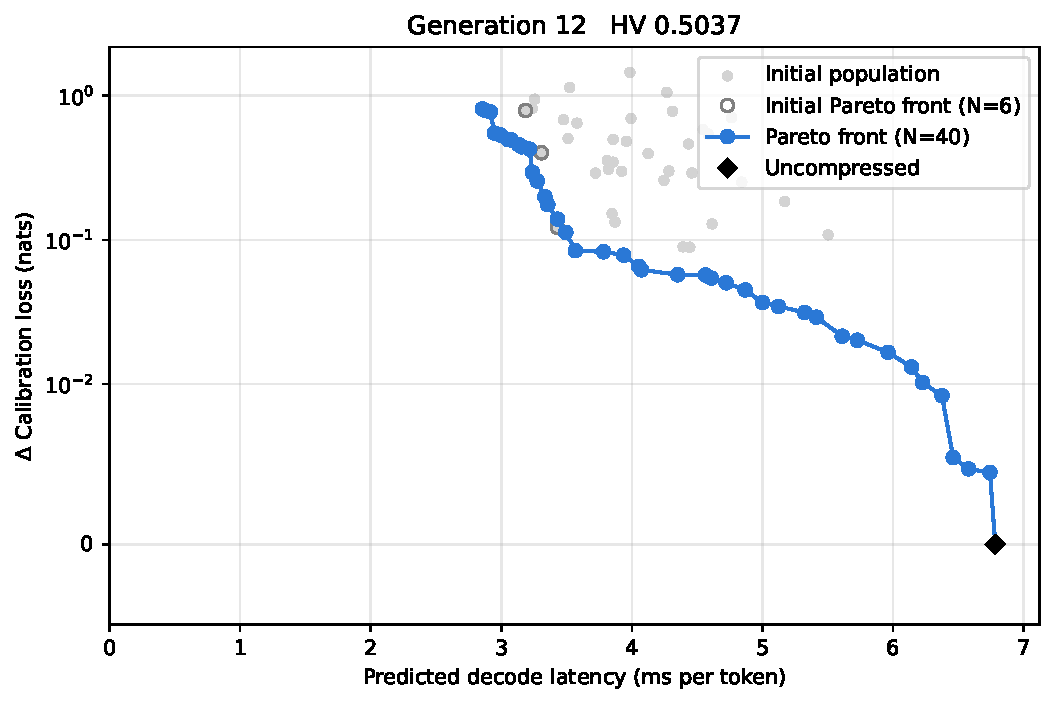
\includegraphics[width=\linewidth]{figures/front_2obj_with_init_pop_log.pdf}
  \caption{Log scale.}
\end{subfigure}\hfill
\begin{subfigure}{0.49\linewidth}
  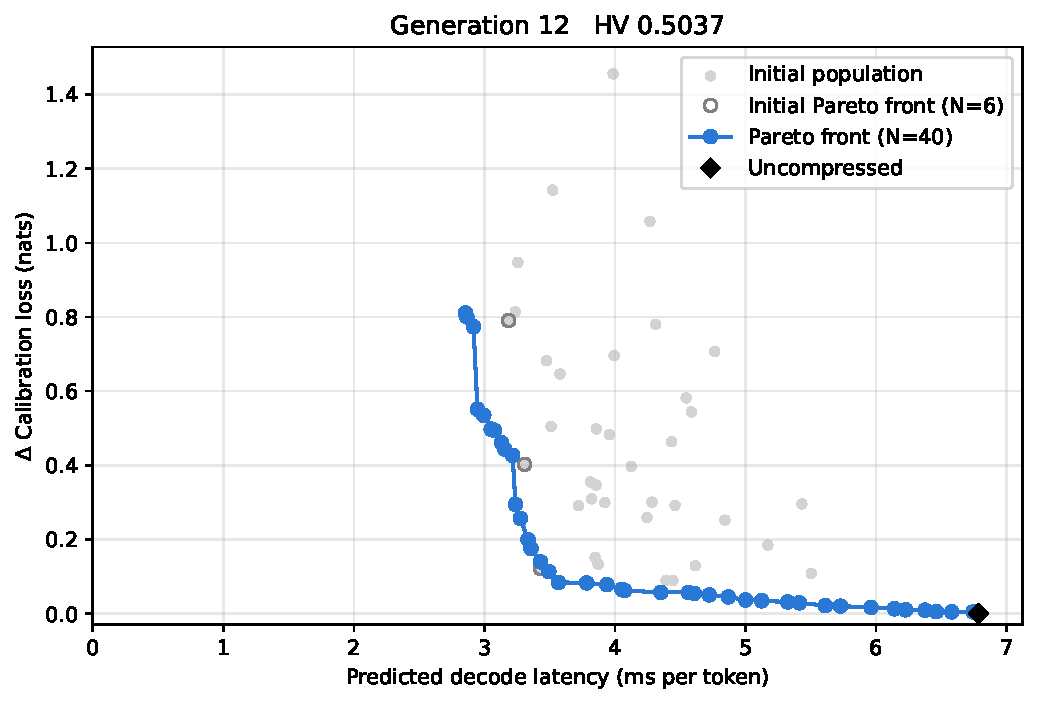
\includegraphics[width=\linewidth]{figures/front_2obj_with_init_pop_linear.pdf}
  \caption{Linear scale.}
\end{subfigure}
\caption{Two-objective search: initial population (grey), initial front (hollow) and final front after
12 generations, with the loss on a log scale (linear below 0.01 nats) and on a linear scale.}
\label{fig:front2}
\end{figure}

\begin{figure}[htbp]
\centering
\begin{subfigure}{0.49\linewidth}
  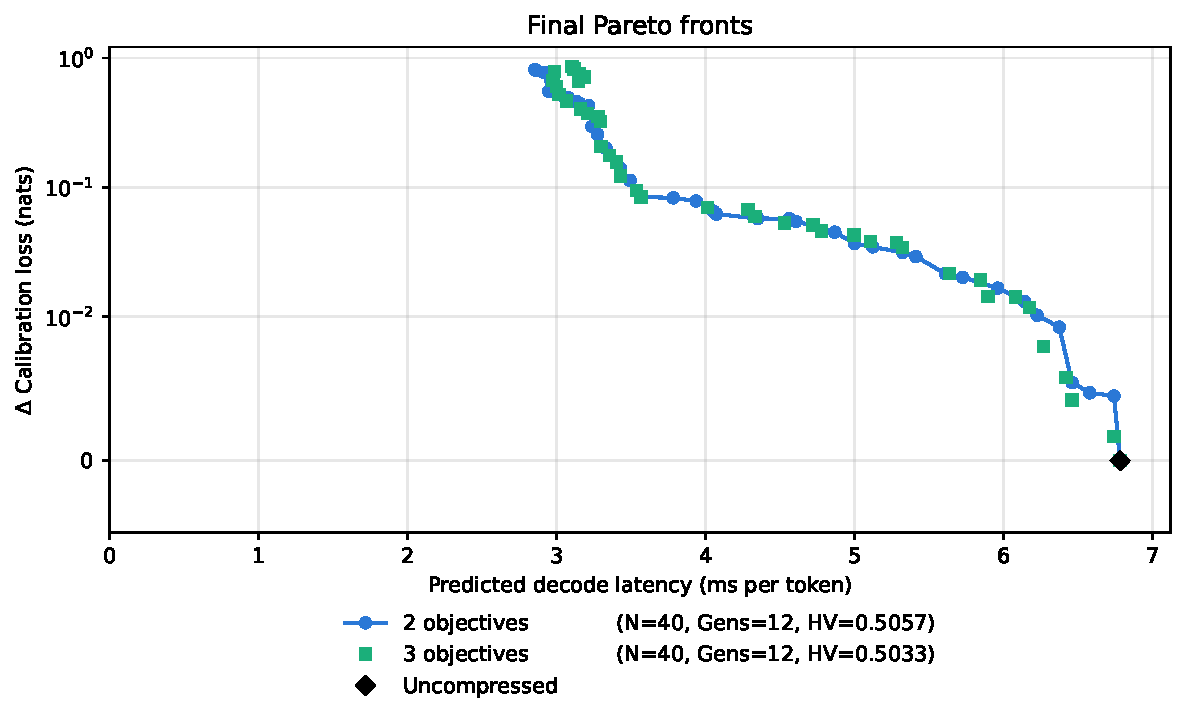
\includegraphics[width=\linewidth]{figures/fronts_latency_log.pdf}
  \caption{Latency, log scale.}
\end{subfigure}\hfill
\begin{subfigure}{0.49\linewidth}
  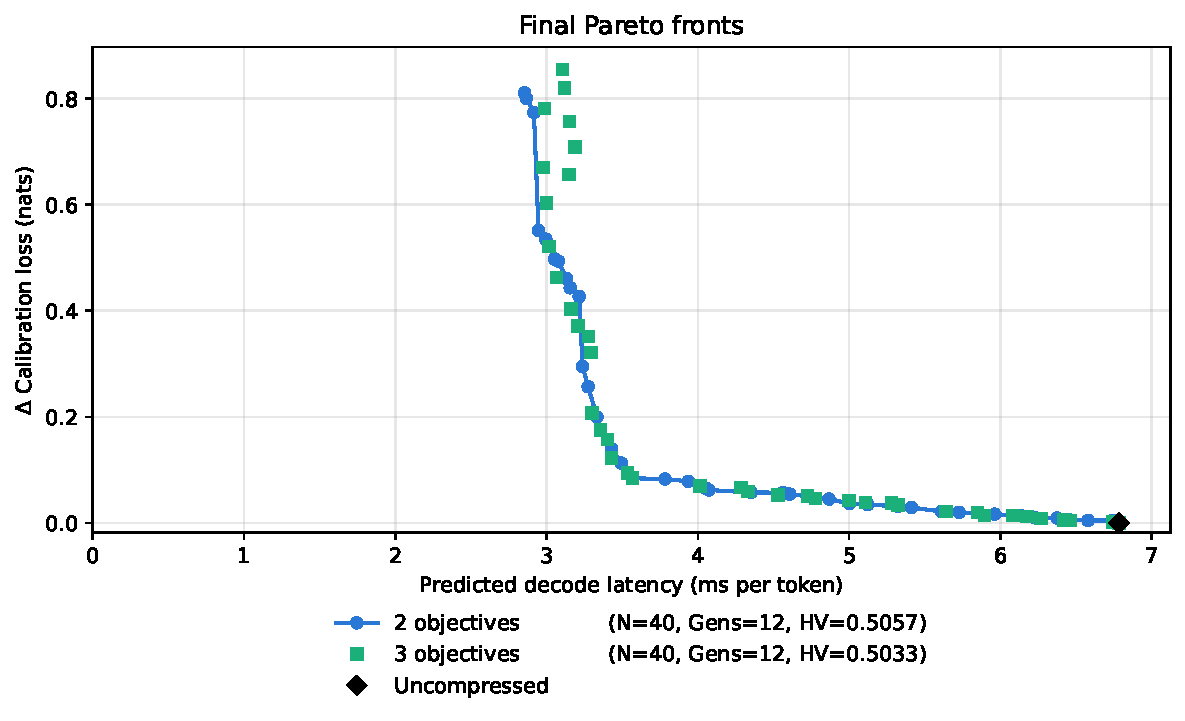
\includegraphics[width=\linewidth]{figures/fronts_latency_linear.pdf}
  \caption{Latency, linear scale.}
\end{subfigure}\\[6pt]
\begin{subfigure}{0.49\linewidth}
  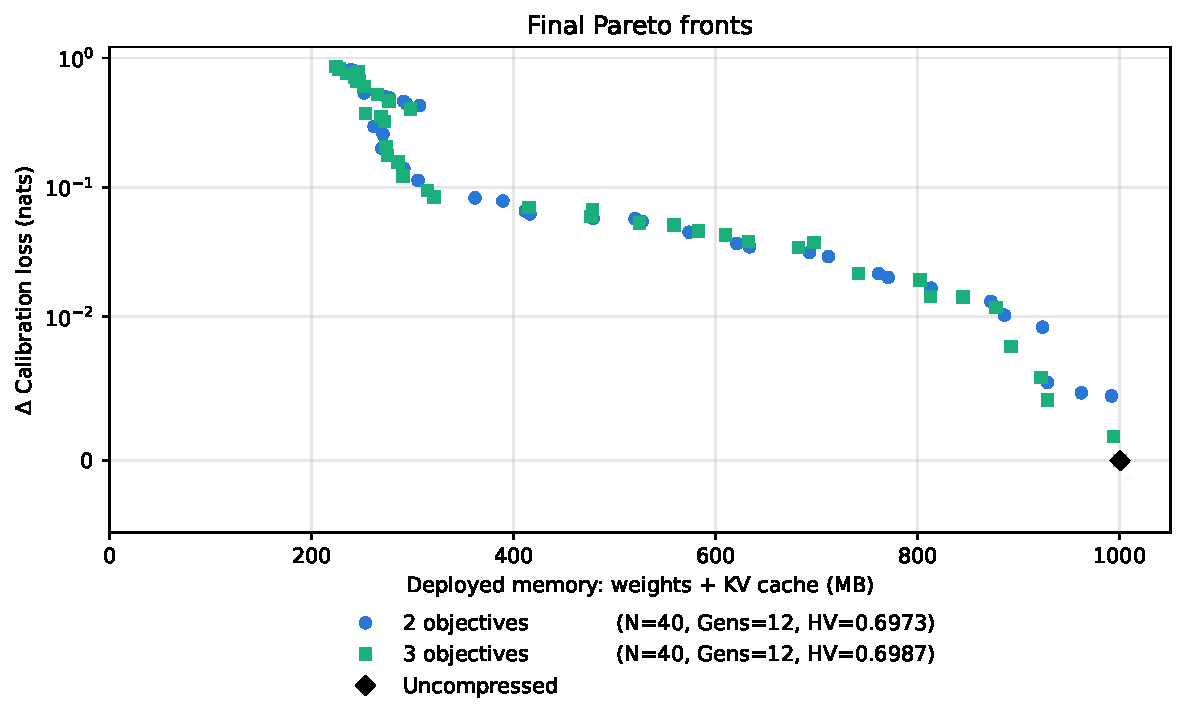
\includegraphics[width=\linewidth]{figures/fronts_memory_log.pdf}
  \caption{Memory, log scale.}
\end{subfigure}\hfill
\begin{subfigure}{0.49\linewidth}
  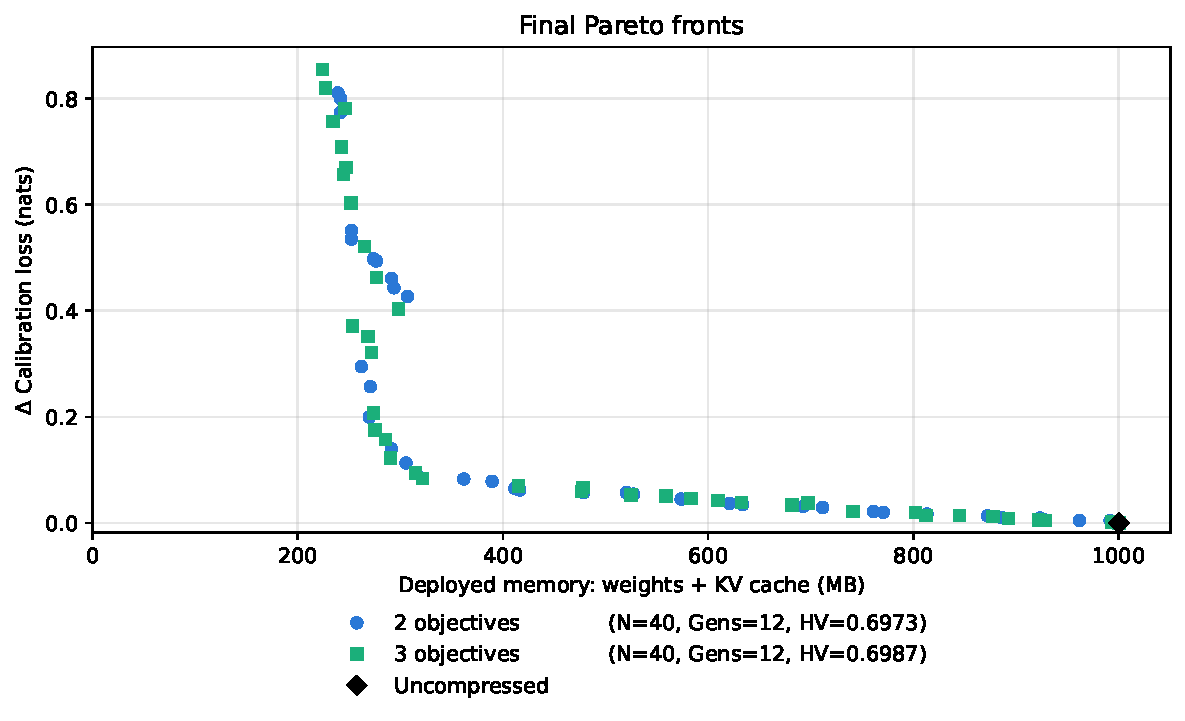
\includegraphics[width=\linewidth]{figures/fronts_memory_linear.pdf}
  \caption{Memory, linear scale.}
\end{subfigure}
\caption{Final fronts of the two searches: loss against predicted decode latency (top) and against
deployed memory (bottom), on a log scale (linear below 0.01 nats, left) and a linear scale (right). A
front is drawn as a line only in the objectives it optimized; elsewhere its points are not ordered
along the axis.}
\label{fig:fronts}
\end{figure}

\subsection{Test perplexity}
Table~\ref{tab:test} lists the test perplexity of the scored points, and Figure~\ref{fig:test} shows
WikiText-2 against latency. The ranking of the calibration loss carries over to both test sets. The
knee of the front, int4 everywhere, costs 10\% WikiText-2 and 9\% C4 perplexity for a
$1.9\times$ faster decode step and $3.1\times$ less memory.

\begin{table}[htbp]
\centering
\small
\begin{tabular}{lrrrrrr}
\toprule
Search & Latency (ms) & Memory (MB) & Bits/weight & $\dloss$ (nats) & WikiText-2 & C4 \\
\midrule
Uncompressed & 6.78 & 1001 & 16.00 & 0 & 14.33 & 22.33 \\
\midrule
2 obj.  & 5.73 & 771  & 12.28 & 0.020 & 14.67 & 22.80 \\
        & 4.61 & 527  & 8.34  & 0.054 & 15.00 & 23.55 \\
        & 3.57 & 321  & 5.00  & 0.084 & 15.73 & 24.29 \\
        & 3.16 & 294  & 4.60  & 0.443 & 25.57 & 35.59 \\
        & 2.85 & 239  & 3.72  & 0.811 & 39.12 & 51.80 \\
\midrule
3 obj.  & 5.85 & 802  & 12.79 & 0.019 & 14.56 & 22.83 \\
        & 4.53 & 525  & 8.29  & 0.053 & 15.40 & 23.42 \\
        & 3.40 & 286  & 4.42  & 0.157 & 17.18 & 26.78 \\
        & 3.15 & 234  & 3.59  & 0.757 & 44.46 & 54.86 \\
        & 2.98 & 247  & 3.84  & 0.670 & 32.87 & 49.46 \\
\bottomrule
\end{tabular}
\caption{Test perplexity (32 windows of 2048 tokens each) of the uncompressed model and of points of the
final fronts of the two searches.}
\label{tab:test}
\end{table}

\begin{figure}[htbp]
\centering
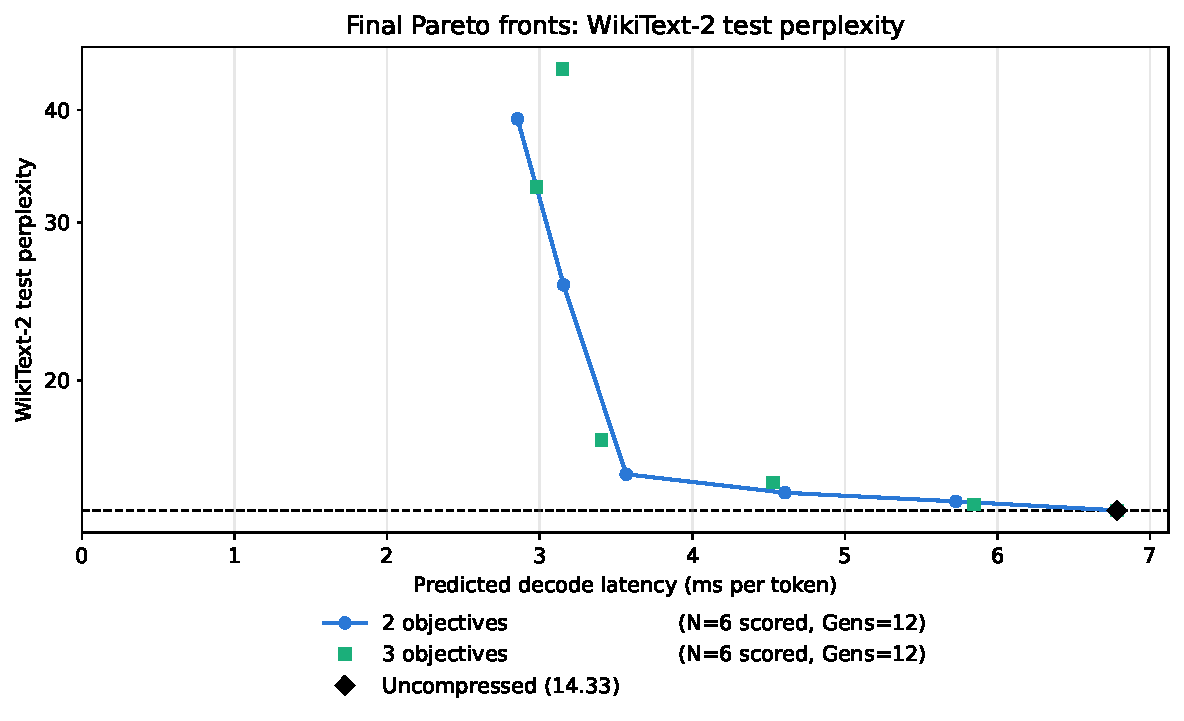
\includegraphics[width=0.62\linewidth]{figures/test_wikitext2_latency.pdf}
\caption{WikiText-2 test perplexity of the scored points against predicted decode latency.}
\label{fig:test}
\end{figure}

\subsection{Two objectives against three}
To compare the scenarios, both final fronts and every generation's front are evaluated in all three
objectives with one normalization: each objective is divided by the worst value over the initial fronts
of both runs, $(0.814\ \text{nats},\ 6.78\ \text{ms},\ 1000.6\ \text{MB})$, with reference point
$(1,1,1)$. The same is done in the two two-dimensional projections. Table~\ref{tab:hv} and
Figure~\ref{fig:hv} show the results.

\begin{table}[htbp]
\centering
\small
\begin{tabular}{rcccccc}
\toprule
Objectives & \multicolumn{2}{c}{\{loss, latency, memory\}} & \multicolumn{2}{c}{\{loss, latency\}} & \multicolumn{2}{c}{\{loss, memory\}} \\
\cmidrule(lr){2-3}\cmidrule(lr){4-5}\cmidrule(lr){6-7}
Generation & 2 obj. & 3 obj. & 2 obj. & 3 obj. & 2 obj. & 3 obj. \\
\midrule
1  & 0.3302          & 0.3302 & 0.4550          & 0.4550 & 0.6504          & 0.6504 \\
2  & \textbf{0.3335} & 0.3313 & \textbf{0.4654} & 0.4587 & \textbf{0.6650} & 0.6555 \\
3  & \textbf{0.3375} & 0.3333 & \textbf{0.4676} & 0.4668 & \textbf{0.6696} & 0.6671 \\
4  & \textbf{0.3444} & 0.3398 & \textbf{0.4786} & 0.4755 & \textbf{0.6815} & 0.6691 \\
5  & \textbf{0.3500} & 0.3461 & \textbf{0.4877} & 0.4836 & \textbf{0.6833} & 0.6757 \\
6  & \textbf{0.3511} & 0.3492 & \textbf{0.4893} & 0.4876 & \textbf{0.6837} & 0.6788 \\
7  & \textbf{0.3584} & 0.3539 & \textbf{0.4967} & 0.4941 & \textbf{0.6892} & 0.6845 \\
8  & \textbf{0.3622} & 0.3564 & \textbf{0.5000} & 0.4974 & \textbf{0.6942} & 0.6870 \\
9  & \textbf{0.3638} & 0.3611 & \textbf{0.5025} & 0.4998 & \textbf{0.6946} & 0.6939 \\
10 & \textbf{0.3651} & 0.3633 & \textbf{0.5050} & 0.5020 & \textbf{0.6961} & 0.6960 \\
11 & \textbf{0.3655} & 0.3639 & \textbf{0.5056} & 0.5026 & 0.6971          & \textbf{0.6974} \\
12 & \textbf{0.3655} & 0.3646 & \textbf{0.5057} & 0.5033 & 0.6973          & \textbf{0.6987} \\
\bottomrule
\end{tabular}
\caption{Hypervolume of each generation's front with one shared normalization, in all three objectives
and in the two projections. Generation 1 is identical because both searches start from the same
population.}
\label{tab:hv}
\end{table}

\begin{figure}[htbp]
\centering
\begin{subfigure}{0.72\linewidth}
  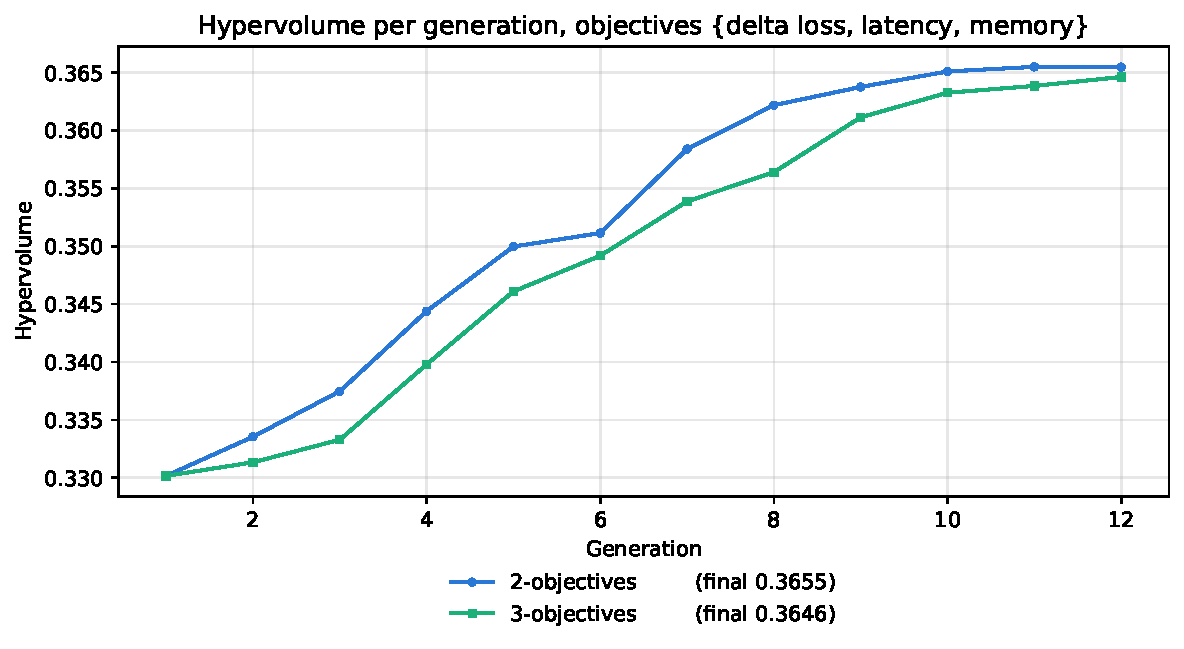
\includegraphics[width=\linewidth]{figures/hv_3d.pdf}
  \caption{\{loss, latency, memory\}.}
\end{subfigure}\\[6pt]
\begin{subfigure}{0.49\linewidth}
  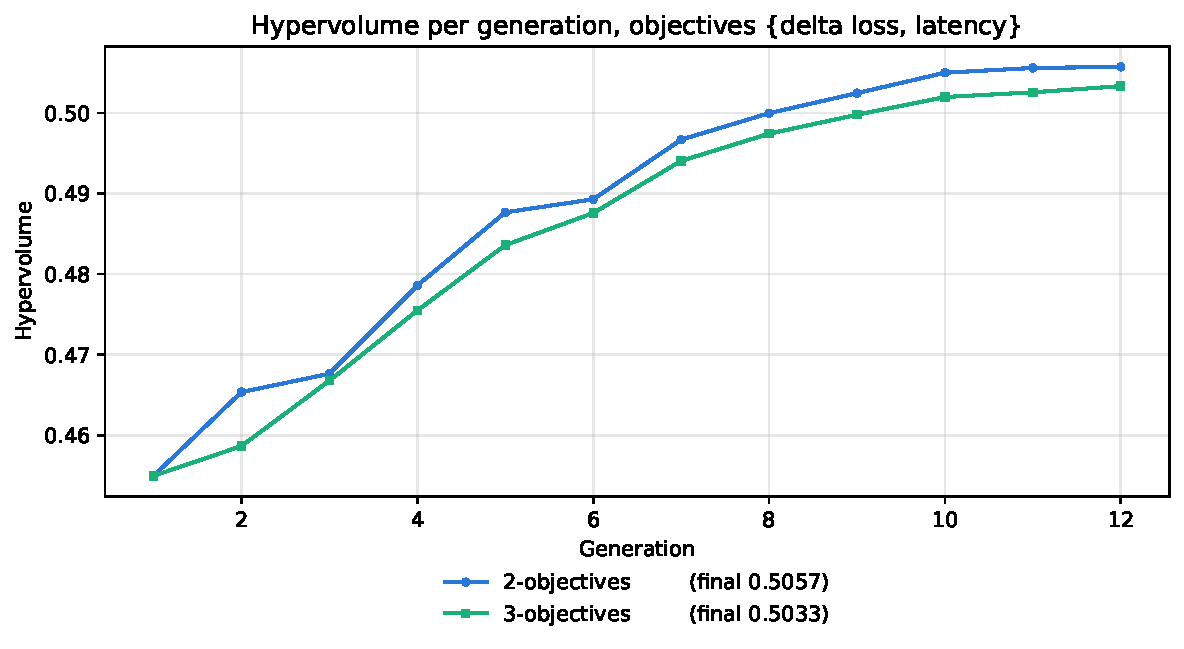
\includegraphics[width=\linewidth]{figures/hv_latency.pdf}
  \caption{\{loss, latency\}.}
\end{subfigure}\hfill
\begin{subfigure}{0.49\linewidth}
  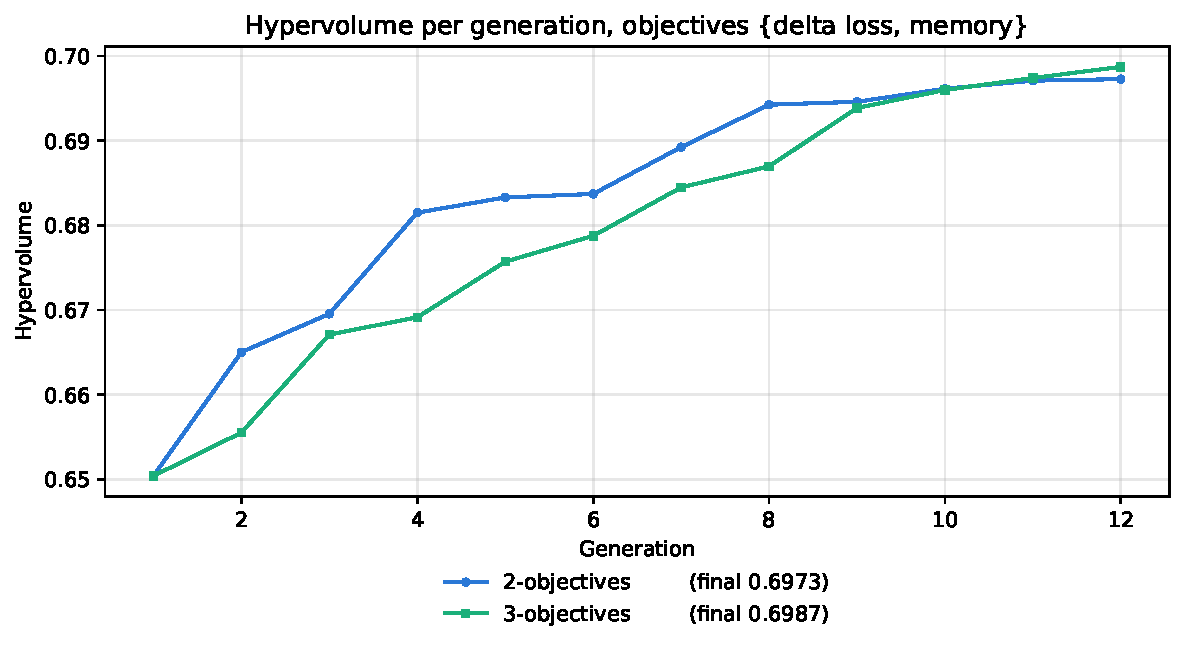
\includegraphics[width=\linewidth]{figures/hv_memory.pdf}
  \caption{\{loss, memory\}.}
\end{subfigure}
\caption{Hypervolume per generation of the two searches with one shared normalization: in all three
objectives (a), and in the projections \{loss, latency\} (b) and \{loss, memory\} (c).}
\label{fig:hv}
\end{figure}

\noindent Three observations:
\begin{itemize}
  \item \textbf{In all three objectives, the two-objective search is ahead in every generation}, by up
        to 1.6\% at generation 8 and by 0.25\% at the end. The ordering holds with a run-independent box
        (the $\dloss$ limit and the uncompressed latency and memory as the reference point: 0.3795 against
        0.3776) and over every feasible solution each search evaluated, not only its final front (0.3815
        with 76 non-dominated points against 0.3781 with 62).
  \item \textbf{Even in \{loss, memory\},} which only the three-objective search optimizes, the
        two-objective search leads until generation 10; the three-objective search overtakes it at
        generations 11--12, by 0.2\%.
  \item \textbf{The fronts lie on a curve, not a surface} (Figure~\ref{fig:fronts3d}): memory and latency
        decrease together.
\end{itemize}
On this model the third objective is nearly redundant with the second, which is the situation analyzed
by objective reduction \cite{brockhoff2009objective}. A redundant objective adds no trade-off to find
but spreads NSGA-II's diversity preservation over an extra dimension, which slows convergence along the
front that matters. With one seed per scenario, differences of this size are within the usual
seed-to-seed variation and are not significant.

\begin{figure}[htbp]
\centering
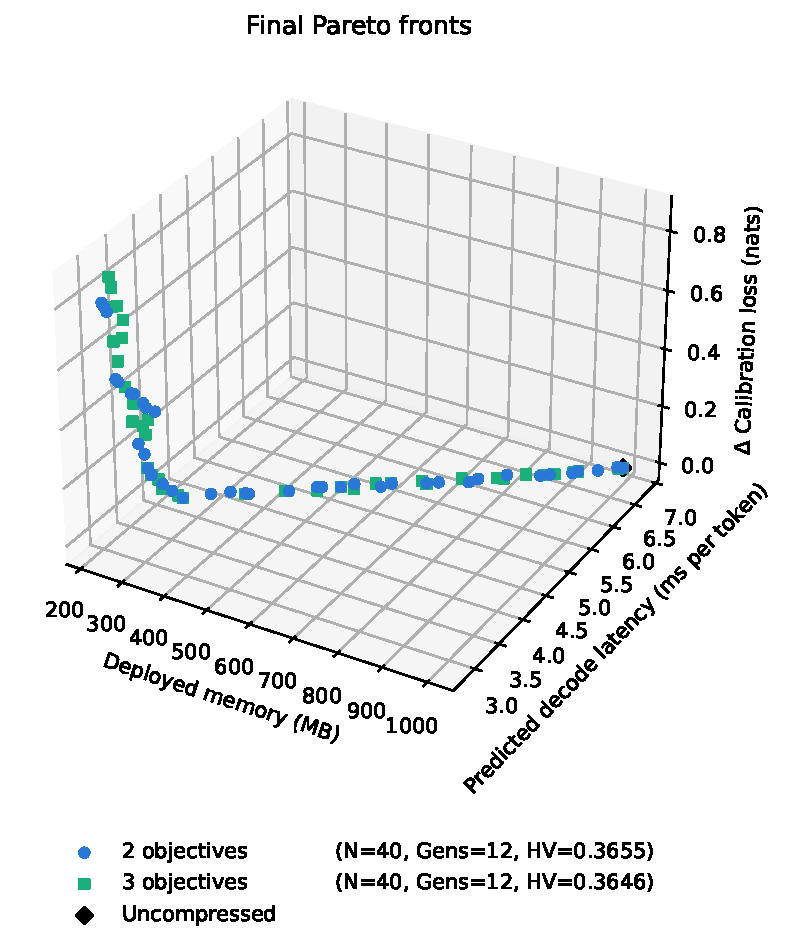
\includegraphics[width=0.66\linewidth]{figures/fronts_3d.pdf}
\caption{Final fronts of both searches in all three objectives. Both lie along a thin curve because
memory and latency decrease together on this model.}
\label{fig:fronts3d}
\end{figure}

% =====================================================================================================
\section{Discussion}
\label{sec:discussion}

\paragraph{When the third objective should matter.}
Latency and memory are nearly collinear on Qwen2.5-0.5B for two reasons: its embedding is tied to the
output head, so compressing it shortens the decode step as well, and its grouped-query attention keeps
the KV cache at 12.6\,MB. nanochat d34 differs on both counts. Its untied embedding of
$65536\times2176$ weights (285\,MB in bf16) costs memory but no decode time, since a lookup reads one
row; a two-objective search has no reason to compress it, while a three-objective search does. Its
multi-head attention keeps 296\,KB of keys and values per token (303\,MB at 1024 tokens), which grows
with the context and the batch. A comparison on d34 would therefore show whether the third objective
earns its cost.

\paragraph{GPU time against wall-clock time.}
The latency objective is GPU time, which is what a runtime with CUDA graphs or a serving engine pays.
Eager PyTorch at batch 1 is limited by the CPU for a model of this size: the deployed models of
Table~\ref{tab:validation} take 23--35\,ms per forward in eager mode against 2.8--6.8\,ms of GPU time,
and the same uncompressed model measured 28.0 and 34.6\,ms in two processes.

\paragraph{Limitations.}
\begin{itemize}
  \item One seed per scenario and 480 evaluations: the comparison of Section~\ref{sec:experiments} is
        indicative only.
  \item The kernel menu is that of this machine: no LUT, 2:4 or fused int8 kernels, and no
        FlashAttention.
  \item The workload is decoding at batch 1; prompt processing is not modeled, and the tinygemm int4
        kernel is 3--5$\times$ slower than bf16 on long prompts (Table~\ref{tab:menu}).
  \item Structurally pruned models are not fine-tuned afterwards, which makes structural pruning look
        worse than it is after a short recovery training \cite{ma2023llmpruner}.
  \item The loss is measured on 8 calibration windows, and the local test sets on 32 windows each.
  \item The latency table belongs to one GPU and one software stack and must be measured on an
        otherwise idle GPU.
\end{itemize}

% =====================================================================================================
\section{Future work}
\label{sec:future}
\begin{itemize}
  \item \textbf{Lookup-table kernels.} With a LUT kernel such as FLUTE \cite{guo2024flute} or the kernels
        of SqueezeLLM \cite{kim2024squeezellm}, non-uniform levels cost nothing at runtime. The per-row
        scale and global codebook of UBQ-ECSQ map directly onto such a kernel, with codebooks of exactly
        $2^b$ entries at 2, 3 or 4 bits.
  \item \textbf{Sparsity and fused kernels on Linux.} 2:4 sparsity \cite{mishra2021sparse} (and int4
        with 2:4 in Sparse-Marlin \cite{frantar2025marlin}), fused int8 activations for prompt-heavy
        workloads \cite{xiao2023smoothquant,ashkboos2024quarot}, and KV-cache quantization for long
        contexts and batches.
  \item \textbf{Per-layer genes.} Decisions per layer instead of per band, seeded by a separable
        sensitivity model solved as a knapsack problem under a latency budget, as in HAWQ-V3
        \cite{yao2021hawqv3}, with the same model screening offspring.
  \item \textbf{A workload objective} that covers prompt processing and generation.
  \item \textbf{Statistics.} Several seeds per scenario, compared by the mean final hypervolume and a
        Mann--Whitney U test.
  \item \textbf{Recovery fine-tuning} of the structurally pruned points of the final front.
\end{itemize}

% =====================================================================================================
\appendix

\section{Measured matrix-product times for Qwen2.5-0.5B}
\label{app:table}

\begin{table}[htbp]
\centering
\small
\begin{tabular}{llrrrr}
\toprule
Matrix ($N\times K$) & Role & bf16 & int4 g32 & int4 g64 & int4 g128 \\
\midrule
$896\times896$ + bias    & $q$                          & 9.6    & 5.0   & 4.7   & 4.6   \\
$128\times896$ + bias    & $k$, $v$                     & 3.6    & 2.5   & 2.5   & 2.5   \\
$896\times896$           & $o$                          & 10.8   & 3.9   & 3.6   & 3.5   \\
$4864\times896$          & gate, up                     & 40.7   & 13.8  & 12.6  & 11.9  \\
$896\times4864$          & down                         & 46.1   & 13.9  & 12.7  & 12.0  \\
$3584\times896$          & gate, up ($\kappa=\tfrac34$) & 30.7   & 10.6  & 9.8   & 9.3   \\
$896\times3584$          & down ($\kappa=\tfrac34$)     & 34.6   & 10.6  & 9.7   & 9.3   \\
$2432\times896$          & gate, up ($\kappa=\tfrac12$) & 21.6   & 7.6   & 7.0   & 6.7   \\
$896\times2432$          & down ($\kappa=\tfrac12$)     & 24.6   & 7.6   & 7.0   & 6.7   \\
$151936\times896$        & output head                  & 1201.5 & 380.0 & 340.9 & 321.3 \\
\bottomrule
\end{tabular}
\caption{GPU time (\us) of one product with a single token. Attention over 1024 cached tokens takes
19.9\us{} per layer (grouped implementation; SDPA: 130.6\us).}
\label{tab:table}
\end{table}

\section{Sublayer removal ranking for Qwen2.5-0.5B}
\label{app:removal}

Loss increase (nats) on 4 calibration windows when one sublayer alone is removed; the search removes
sublayers in this order.
\begin{itemize}
  \item \textbf{Attention}, first eight: layer 18 (0.027), 13 (0.032), 6 (0.035), 19 (0.038), 7 (0.040),
        22 (0.042), 9 (0.043), 11 (0.060); last: 23 (0.342), 0 (2.37), 1 (5.12).
  \item \textbf{MLP}, first eight: layer 12 (0.056), 10 (0.057), 11 (0.069), 9 (0.079), 13 (0.082),
        14 (0.084), 8 (0.095), 18 (0.119); last: 23 (0.537), 2 (2.08), 0 (7.94).
\end{itemize}
The middle layers are the most redundant and the first and last ones the least, in line with
ShortGPT \cite{men2024shortgpt}.

\bibliographystyle{plainnat}
\bibliography{references}

\end{document}
